%%%%%%%%%%%%%%%%%%%%%%%%%%%%%%%%%%%%%%%%%%%%%%%%%%%%%%%%%%%%%%%%%%%%%%%%%%%%%%%%
% experiment.tex: Chapter describing the experiment
%%%%%%%%%%%%%%%%%%%%%%%%%%%%%%%%%%%%%%%%%%%%%%%%%%%%%%%%%%%%%%%%%%%%%%%%%%%%%%%%
\chapter{The Large Hadron Collider and CMS Experiment}
\label{sec:experiment_chapter}
%%%%%%%%%%%%%%%%%%%%%%%%%%%%%%%%%%%%%%%%%%%%%%%%%%%%%%%%%%%%%%%%%%%%%%%%%%%%%%%%
%\subsection{Overview of the Compact Muon Solenoid and Large Hadron Collider}
The CMS experiment was built to detect all ST particles, and to
search for interactions that produced ST particles, like those described in Chapter ~\ref{wrBosonAndHeavyNu}.  The CERN LHC 
collides high-energy protons at the geometric center of the CMS experiment, and the results of proton-proton (pp) 
interactions are recorded.

The results of pp interactions were recorded if any of the following were detected:
\begin{itemize}
	\item one or more energetic charged leptons (electron, muon, tau or their anti-particles)
	\item one or more energetic photons
	\item one or more energetic hadronic jets, each containing at least one hadron
	\item one or more energetic neutrinos\footnote{the presence of neutrinos is inferred by measuring a net imbalance in 
		momentum from all detected charged leptons, photons and jets in a collision event.}
	\item combinations thereof
\end{itemize}
Particles produced by pp interactions were detected using a 3.8$\unit{T}$ magnet and four CMS 
sub-detector systems.  The important aspects of each sub-detector system are presented here, a more detailed 
description is given elsewhere \cite{cmsDetectorPaper}.  As shown in Figure \ref{fig:layersOfCMS}, the nominal pp interaction point 
was surrounded by the silicon tracker where charged particles were first detected.  As charged particles traversed
the tracker, mobile electron-hole (e-h) pairs were created along their trajectories.  The tracker detected 
charged particles by counting the number of e-h pairs created.

\begin{figure}[h]
	\centering
	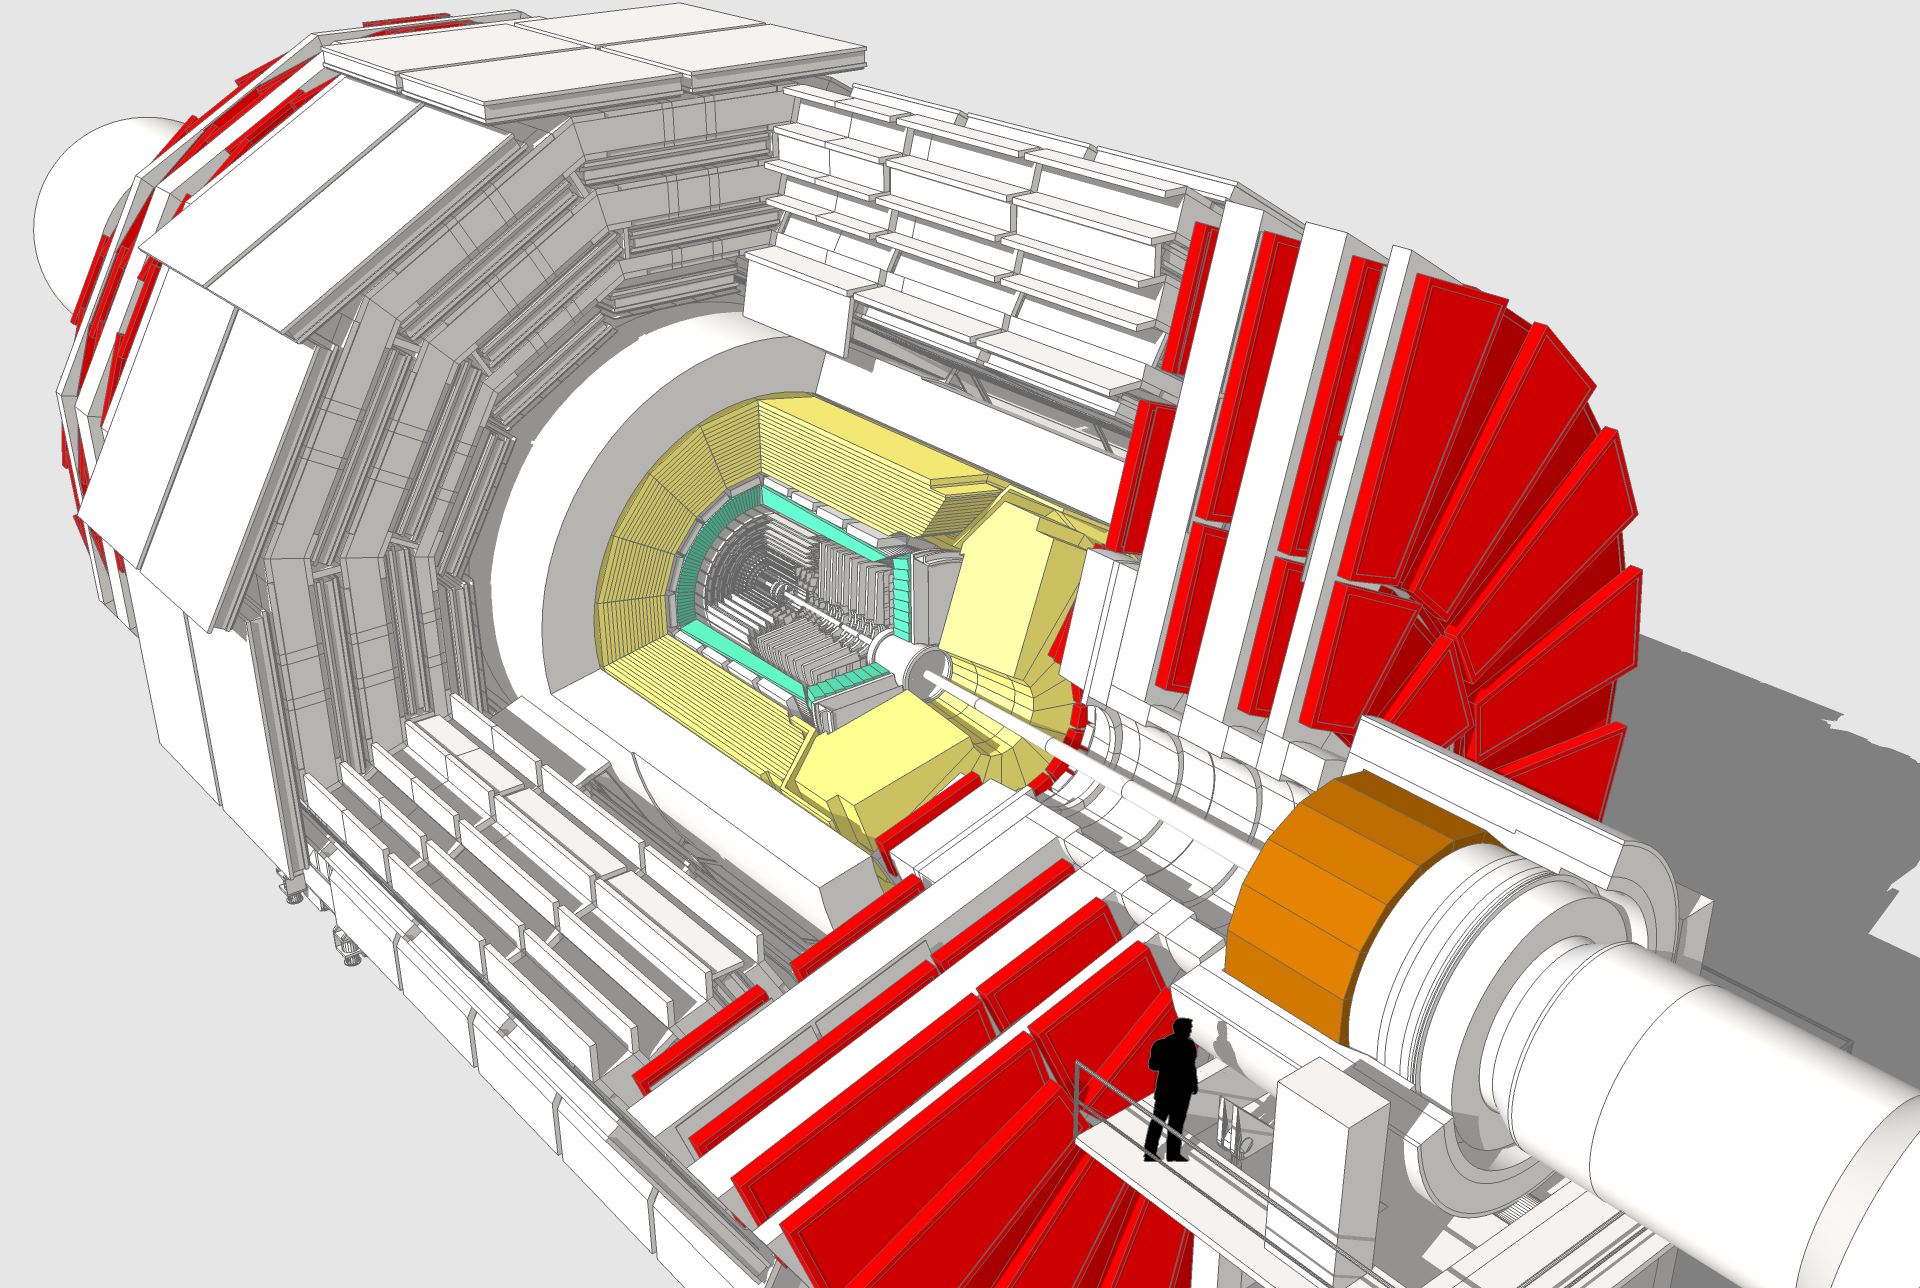
\includegraphics[width=1\textwidth]{figures/cmsDetectorBasic.png}
	\caption{Cut-away view of the entire CMS detector.  Closest to the proton-proton collision/interaction point is the 
		silicon tracker, followed by the Electromagnetic Calorimeter, then the Hadronic Calorimeter, and the 
	magnet.  Outside the magnet solenoid are the muon detectors.}
	\label{fig:layersOfCMS}
\end{figure}


Surrounding the silicon tracker was the lead-tungstate crystal (PbWO$_{4}$) Electromagnetic Calorimeter (ECAL).  
The ECAL was an absorption calorimeter that detected photons, and distinguished electrons and positrons from other charged 
particles detected by the tracker.  Electrons, positrons and photons interacted with lead-tungstate nuclei, 
produced showers of lower energy $e^{\pm}$ that interacted with atomic electrons in PbWO$_{4}$, and subsequently 
emitted visible light through fast ($\lesssim$20 ns) scintillation.  Electrons, positrons and photons produced 
by pp interactions were detected by measuring the visible light produced by PbWO$_{4}$ crystals.

Wrapped around the ECAL was the Hadronic Calorimeter (HCAL).  Built from alternating layers of brass absorber and 
scintillating plastic tiles, the HCAL was a sampling calorimeter that detected hadrons in jets.  Hadrons that 
reached the HCAL interacted with nucleons in brass absorber layers, produced showers of 
lower energy hadrons that interacted with plastic scintillator molecules, which then emitted visible light through 
fast ($\lesssim$10 ns) scintillation.  Hadrons in jets produced by pp interactions were detected by measuring the 
visible light produced by scintillating plastic tiles.

Outside the HCAL was the solenoid magnet that generated a 3.8$\unit{T}$ field.  The magnetic field was generated by running a current of 
$\lesssim$18000 amps through superconducting wire wound into a solenoid.  The wire, made from a niobium alloy, was 
cooled to a superconducting state using a cryogenic system adjacent to the solenoid.  The magnet and its subsystems 
were supported by a structure made mostly from iron, which stopped most particles except muons.

Surrounding the magnet were the muon detectors, which were in a magnetic field with strength between 1 and 3$\unit{T}$.  Three 
different technologies - drift tubes (DT) in the lowest radiation regions, cathode strip chambers (CSC) in higher 
radiation regions, and resistive plate chambers (RPC) in all regions - were used to detect muons.  In these detectors 
muons travelled through pressurized gas chambers and ionized charges from the gas along their 
trajectories.  Within the chambers, electric fields accelerated ionized charges towards conducting wires.  Muons 
were detected by measuring the charge collected by conducting wires.

Due to the enormous rate of diffractive and inelastic pp collisions where energy was detected, a two tiered trigger 
system selected events during collisions for offline reconstruction.  The first tier of the trigger system processed 
information from the ECAL, the HCAL and the muon 
detectors in small regions where high energy particles were detected.  Then, these high energy regions of interest 
were processed by the second tier trigger system.  In the second tier, reconstruction software 
was run in regions of interest to identify charged leptons, photons, jets and neutrinos.  If a pp collision event produced 
one or more reconstructed particles passing second tier energy and quality selections, then all data 
from all four sub-detector systems was read out and used in offline particle reconstruction.

The accelerator that collided protons, the coordinate system used to characterize the kinematics of detected 
particles, the four sub-detector systems and the trigger system are discussed in this chapter.

\section{The Large Hadron Collider}
\label{sec:lhcDescription}
Situated near Geneva, Switzerland and spanning the French-Swiss border, the CERN Large Hadron Collider (LHC) accelerated 
two counter-rotating proton beams in a 27 km circular tunnel \cite{lhcTDR} to an energy of 6.5 $\TeV$ in 2015.  The two beams 
collided at several points along the tunnel, and the CMS experiment was built around one of these points.

Several accelerator stages, shown in Figure \ref{fig:accelComplex}, were used to create each LHC proton beam.  
Each proton beam began as isolated proton bunches ionized from hydrogen gas.  Proton bunches were then accelerated to higher 
energies in 3 accelerator stages before they were injected into the LHC.  Once enough proton bunches were 
collected in the LHC (up to $\sim$2300 for each beam), the LHC created two proton beams with proton bunches separated by 
25\ns, and accelerated both beams to an energy of 6.5 $\TeV$.

\begin{figure}[ht]
	\centering
	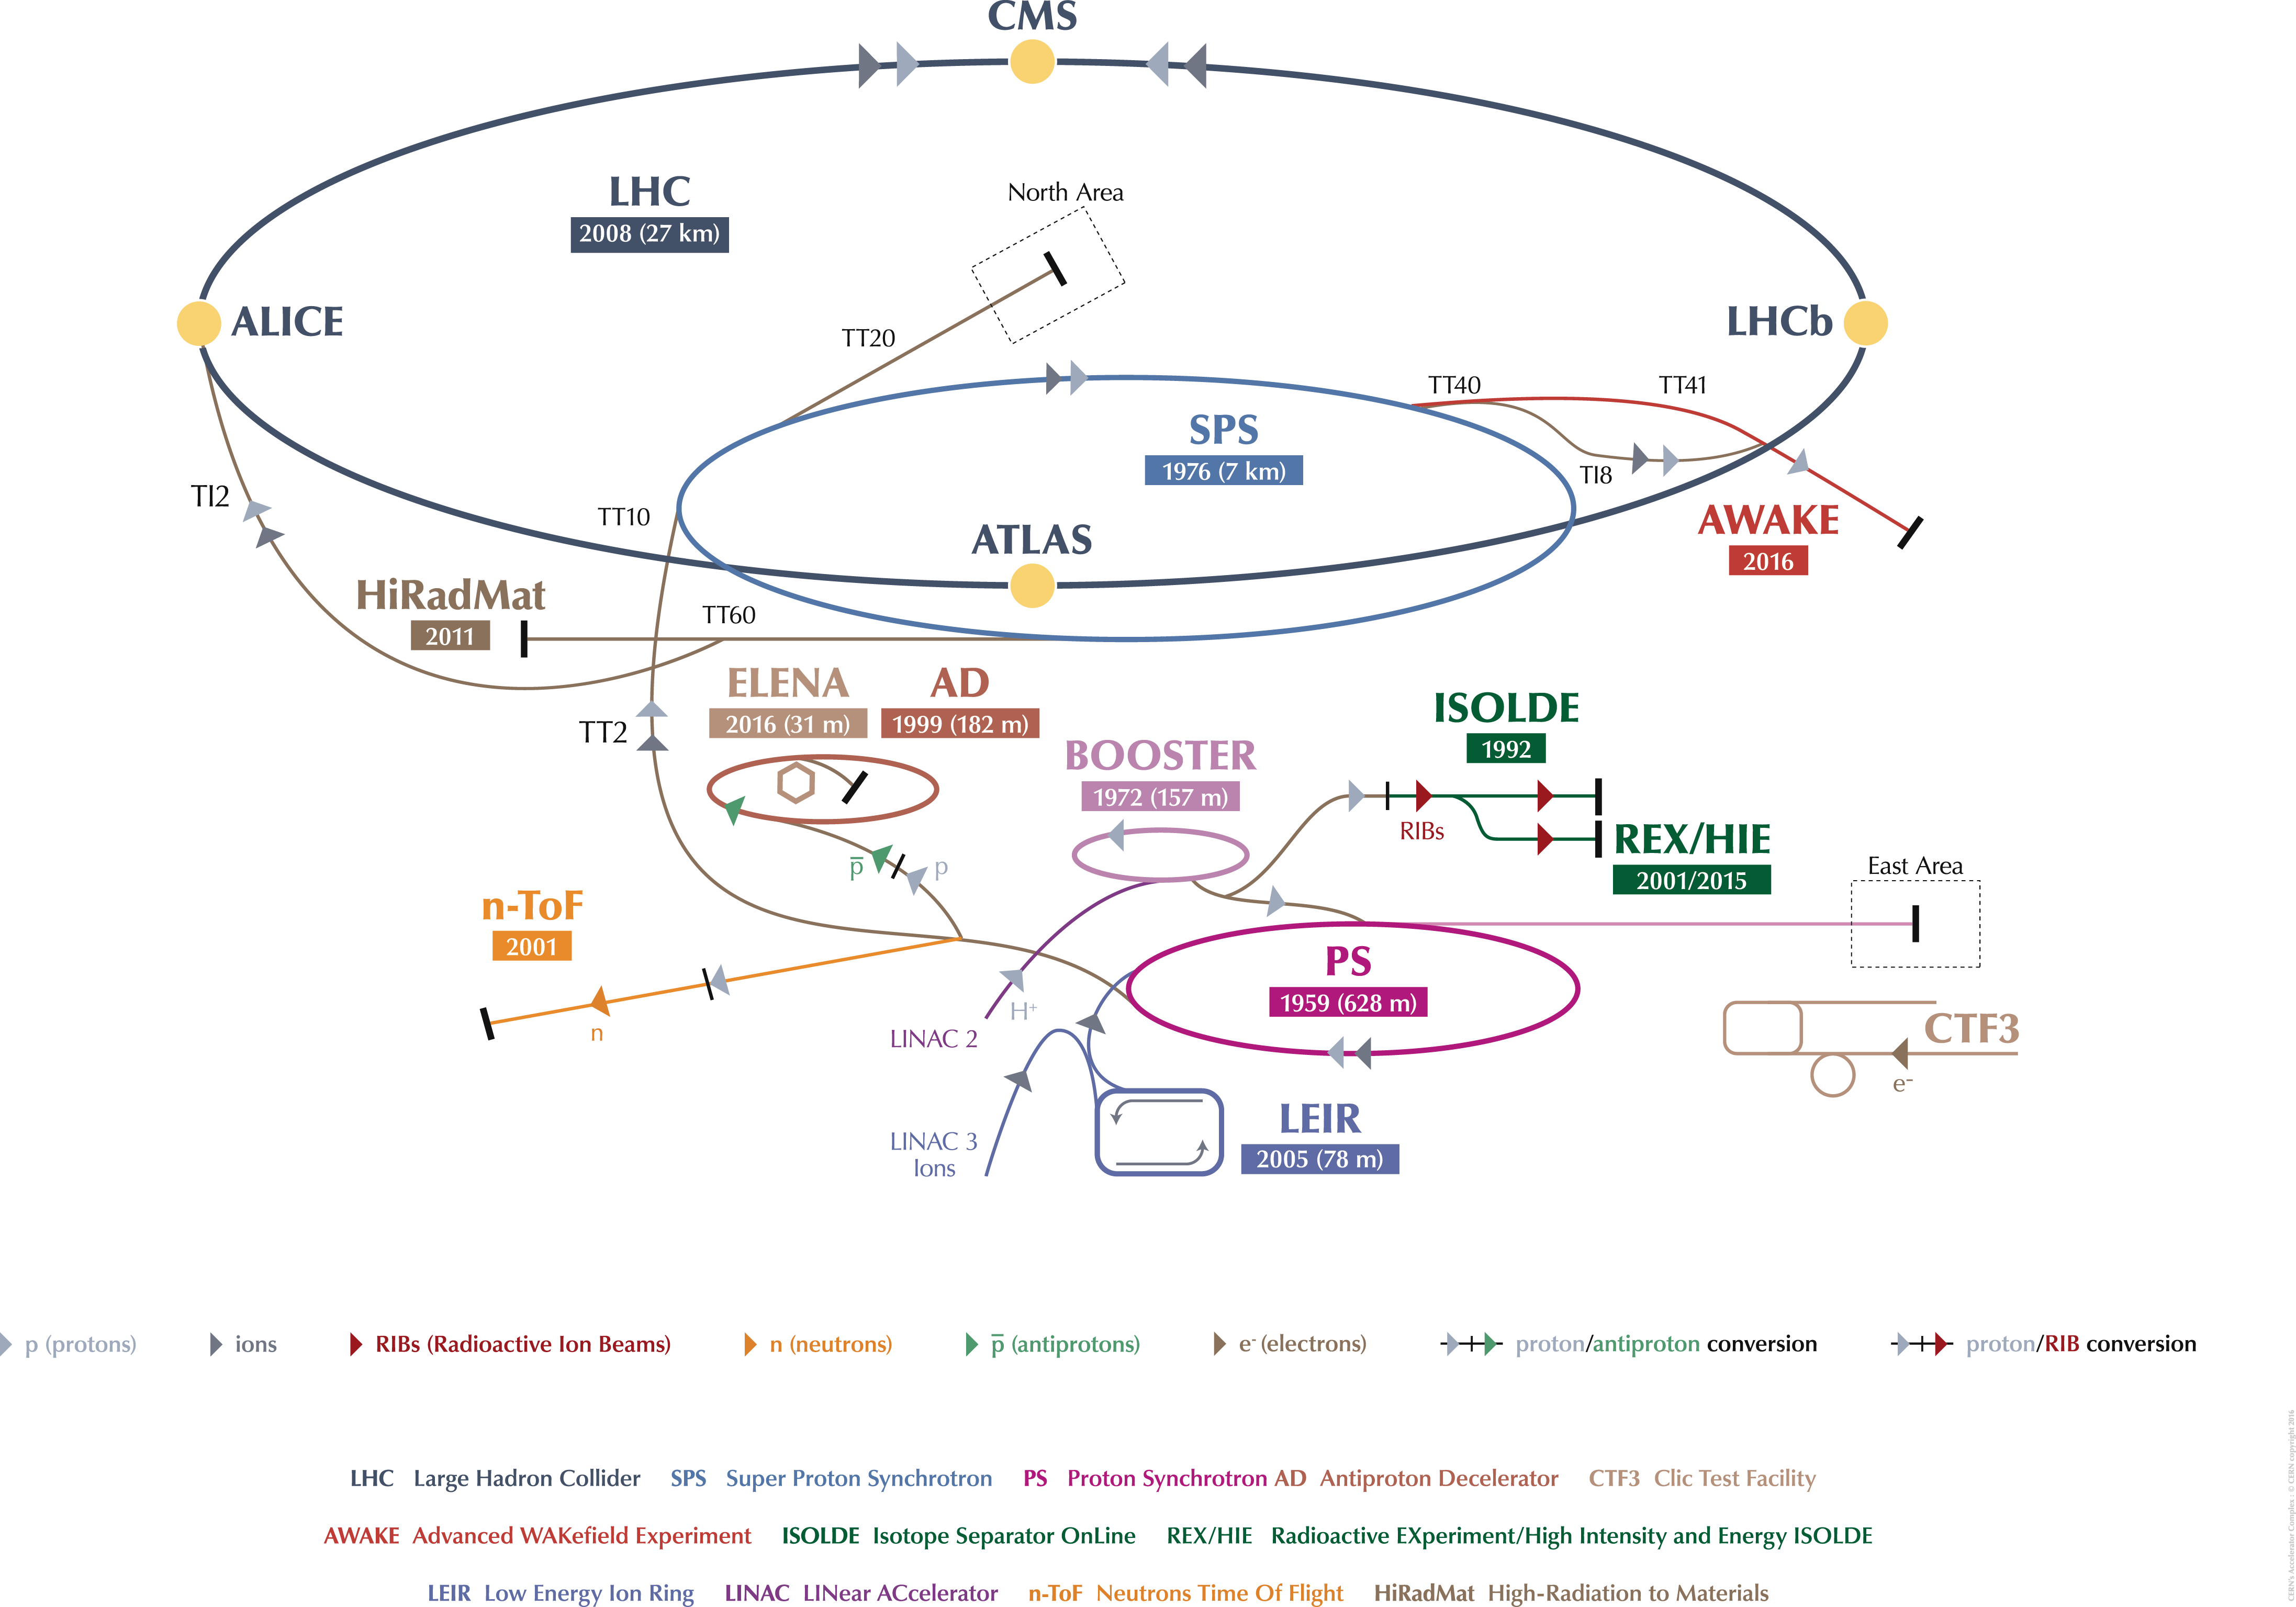
\includegraphics[width=1\textwidth]{figures/CERNAcceleratorComplex.png}
	\caption{The CERN accelerator complex.  Protons are ionized from hydrogen, then are accelerated to higher 
	energies by LINAC 2, the PS, and finally the SPS before entering the LHC.  From CERN.}
	\label{fig:accelComplex}
\end{figure}


In the LHC tunnel, superconducting radio-frequency (RF) cavities accelerated proton bunches, and magnets steered and 
focused the beams towards the collision point at the heart of CMS.  
During 2015 data taking the LHC collided protons at intensities approaching $6 \times 10^{33} \frac{1}{cm^{2}s}$ ($\sim 0.02 \frac{1}{fb\thickspace hr}$).  

\section{The CMS Coordinate System and Kinematic Variables}
\label{sec:coordinateSystemAndKinematicVars}
A right-handed coordinate system and kinematic variables are used to characterize the kinematics of detected particles.  
The coordinate system defines the $z$ axis pointing in the counter-clockwise direction, the $y$ axis 
points at the surface, and the $x$ axis points at 
the LHC ring center, as shown in Figure \ref{fig:cmsAndCoordinateSystem}.  In this coordinate system particle 
trajectories are described using two angular variables, $\phi$ and $\eta$, that are defined 
in separate coordinate planes.  $\phi$ is the angle in the $x-y$ plane, and spanned values between 0 and $2\pi$.  
$\theta$ is defined in the $y-z$ plane, and is 0 ($\frac{\pi}{2}$) when pointing along the $z$ ($y$) axis.  
$\theta$ is transformed into pseudorapidity $\eta$ through the following function:

\begin{equation}
	\eta \equiv -\ln{\tan{\frac{\theta}{2}}}
\end{equation}


\begin{figure}[ht]
	\centering
	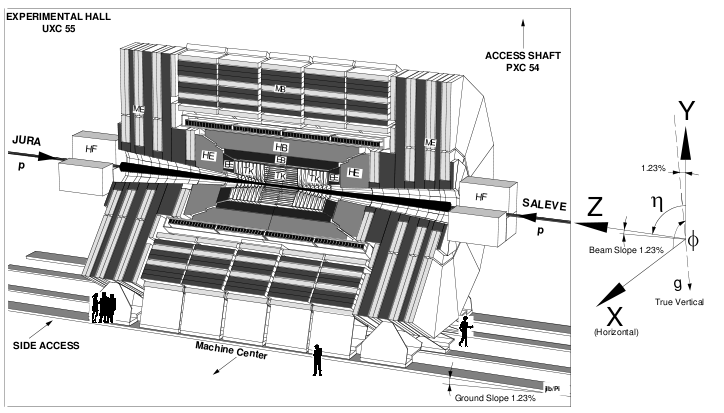
\includegraphics[width=1\textwidth]{figures/cmsDetectorAndCoordinateSystem.png}
	\caption{All CMS detector components and the coordinate system used to describe particle kinematics.}
	\label{fig:cmsAndCoordinateSystem}
\end{figure}

$\eta$ of 0 points along the $y$ axis, while $\eta$ of $\infty$ points along the $z$ axis.
An equivalent definition of pseudorapidity in terms of the particle energy E and longitudinal 
momentum $p_{z}$ in the massless particle limit is:

\begin{equation}
	\eta \equiv \frac{1}{2}\ln{\frac{E+p_{z}}{E-p_{z}}}
\end{equation}

Pseudorapidity is used to describe particle trajectories instead of the angle $\theta$ for several reasons.  Particles 
produced by pp interactions were often boosted along the $z$ axis, but the degree of boost was never well 
defined because the momenta of the interacting partons was unknown.  This boost affected the 
trajectories of particles in $\theta$, but did not affect particle trajectories in $\eta$.  In 
addition, the particles that caused radiation damage in CMS sub-detector systems were produced at 
a rate that scaled linearly with $\eta$.  Thus, in discussions where radiation damage or particle 
isolation played a role, ideas could be more clearly articulated using $\eta$.

The main variables used to quantify particle energies are transverse energy 
$\Et \equiv E/\cosh{\eta}$ and transverse momentum $\pt \equiv |p|/\cosh{\eta}$.  The silicon tracker and muon detectors measure $\pt$, 
while the calorimeters measure $\Et$.  The distance between 
a particle and another point in the $(\eta, \phi)$ space is measured as $\Delta R \equiv \sqrt{\eta^{2} + \phi^{2}}$.  
%Transverse momentum $\pt$, the component of momentum perpendicular to the proton beam axis, and transverse energy $\Et$, the 
%analogous form of energy, were used because both were insensitive to the unknown $z$ momenta of the interacting partons.  

\section{The Silicon Tracker}
\label{sec:siTrackerDescription}
The silicon tracker consisted of silicon pixel and strip detectors that detected charged particles and measured their 
momenta by tracking charged particles as they traversed the magnetic field, and identified interaction vertices.  Closest 
to the beam axis was the pixel detector, which used silicon pixels to pinpoint pp interaction vertices with $\mu$m precision.  
Surrounding the pixel detector was the strip detector, which used silicon strips to measure charged particle momenta with 
a resolution of a few percent.  Charged particles produced within the tracker acceptance of $|\eta| < 2.5$ generated an 
analog signal that was detected and stored in an analog memory until it was readout or discarded.

to the beam axis was the pixel detector, which used $\approx$1 m$^{2}$ of silicon divided into 100 $\times$ 150 $\mu$m$^{2}$ 
silicon pixels to pinpoint pp interaction vertices with $\mu$m precision.  Surrounding the pixel detector was the strip 
detector, which used 200 m$^{2}$ of silicon divided into silicon strips\footnote{The strip size varied with $\eta$ and 
distance away from the beam axis - the strip width was between 80 and 180 $\mu$m, and the strip length was between 
12 and 16 cm.} to measure charged particle momenta with a resolution of a few percent.  Charged particles produced within 

The pixel detector was built from $\approx$1 m$^{2}$ of silicon divided into 100 $\times$ 150 $\mu$m$^{2}$ silicon detectors.  
In the barrel region ($0 < |\eta| < 1.2$), individual silicon detectors were assembled in three concentric cylindrical shells 
centered on the $z$ axis.  In the endcap region ($1.2 < |\eta| < 2.5$), two layers of silicon detectors were 
installed in a turbine pattern as shown in Figure \ref{fig:pixelTracker} \cite{pixelCommissioning}.  These pixel 
layers provided up to 3 measurements for every track, and primarily were used to reconstruct interaction 
vertices.

\begin{figure}[ht]
	\centering
	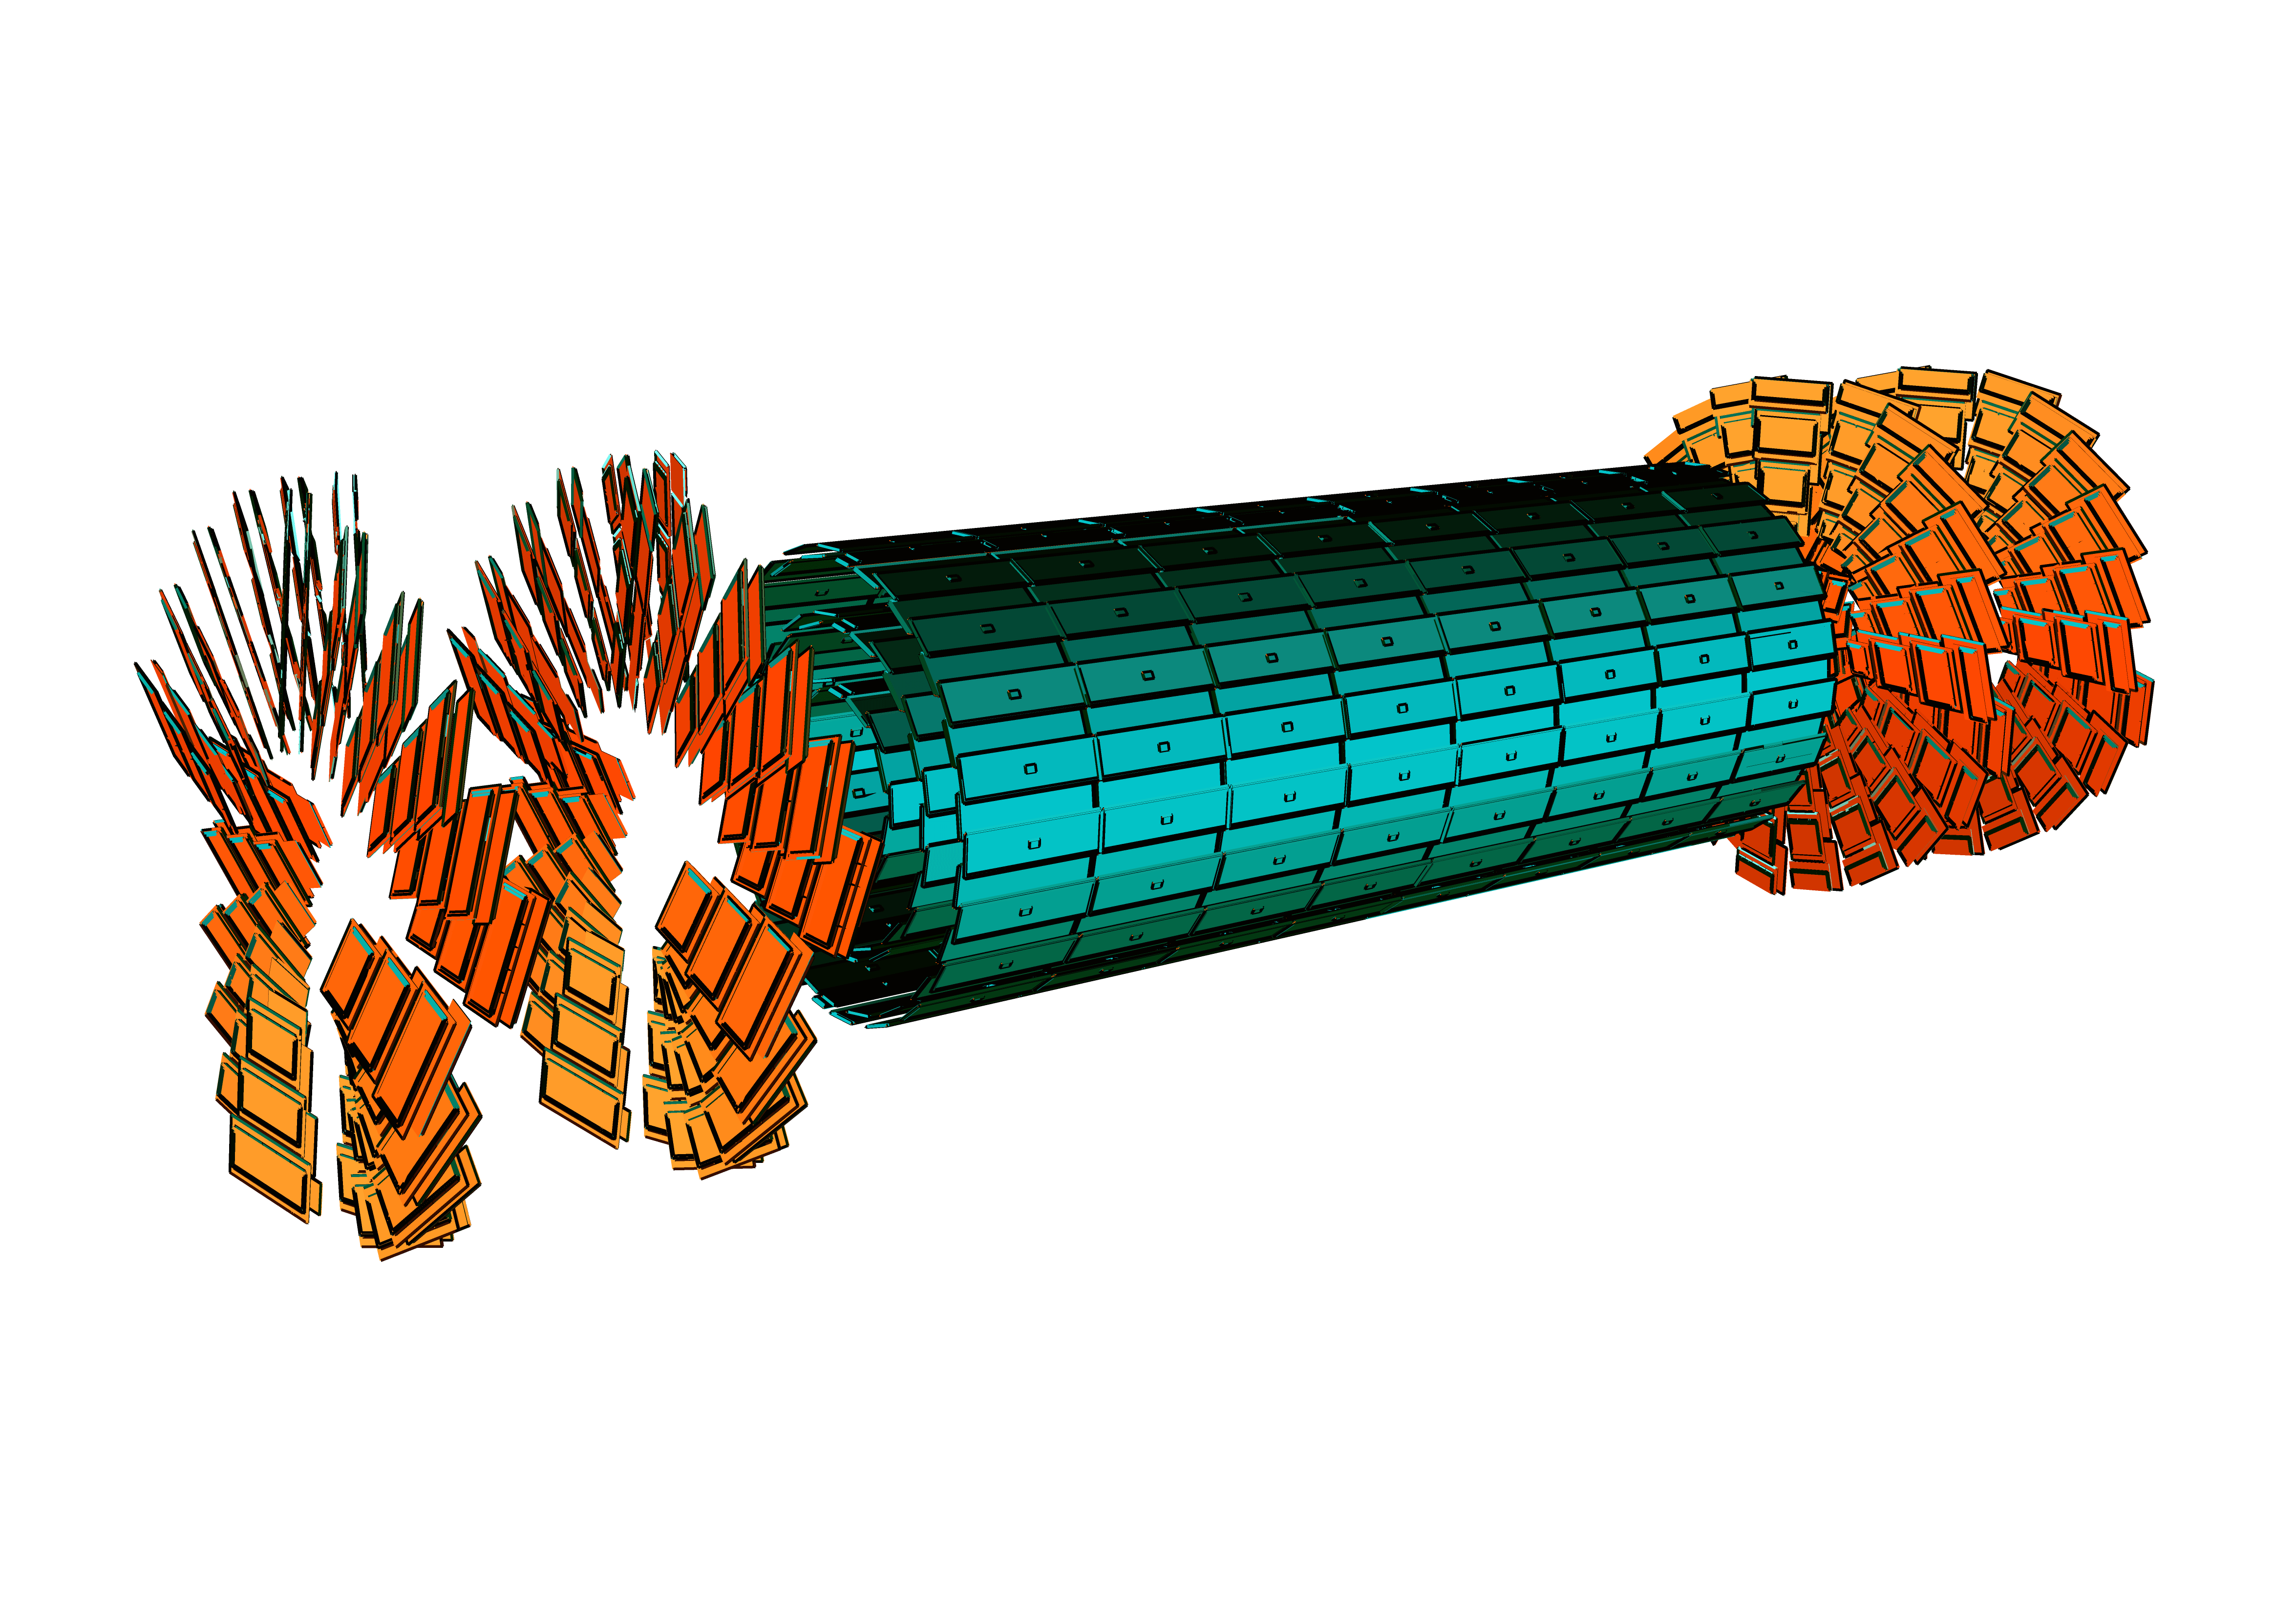
\includegraphics[width=0.8\textwidth]{figures/pixelDetectorSchematic.png}
	\caption{The barrel and endcap sections of the pixel detector.}
	\label{fig:pixelTracker}
\end{figure}

Located outside the pixel detector, the strip detector was constructed with 200 m$^{2}$ of silicon divided into larger silicon detectors\footnote{The strip size varied with $\eta$ and 
distance away from the beam axis - the strip width was between 80 and 180 $\mu$m, and the strip length was between 12 and 16 cm.} organized 
into four structures based on $|\eta|$, and distance from the interaction point.  In the barrel region, silicon detectors 
were used to build 10 concentric cylindrical shells.  In the endcap region, silicon detectors 
were arranged in 12 disks, as shown in Figure \ref{fig:stripTracker} \cite{cmsTDR}, with some overlap in $|\eta|$ with the 
barrel region silicon detectors.  The strip detector provided 5 to 14 measurements for every track, and was primarily used to 
measure the momenta of charged particles.

\begin{figure}[ht]
	\centering
	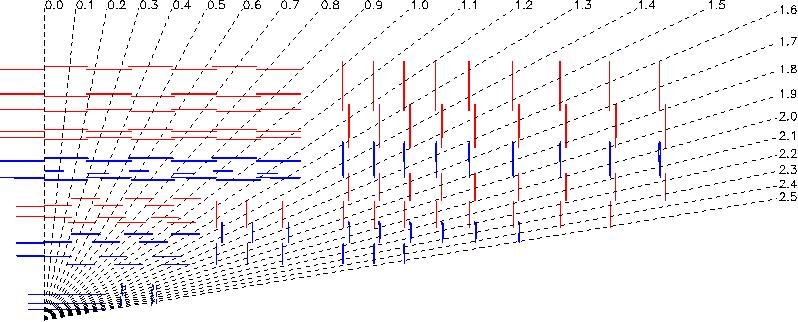
\includegraphics[width=0.8\textwidth]{figures/siliconStripAndPixelDetectorTwoDimView.png}
	\caption{The barrel and endcap sections of the strip detector for $\eta \geq 0.$ and one quadrant of $\phi$.  
	The pixel detector is shown to scale in the bottom left corner.}
	\label{fig:stripTracker}
\end{figure}

The signal from a charged particle traversing a detector was measured by readout modules connected to groups of pixels or 
strips\footnote{$\sim$16000 readout modules were connected to 66 million pixels, and $\sim$15400 readout modules were connected 
to 9.6 million strips.}.

The tracker performance depended on the number of tracks in a collision event, and the momenta of 
charged particles.  The tracker measured the position of an interaction vertex with a resolution that improved when more 
tracks were associated with the vertex.  The search presented in this thesis used collision events where the tracker 
measured the coordinate of the $\ell\ell jj$ interaction vertex with a resolution better than 12$\mu$m in any direction \cite{trackerPerformanceInCollisions}.  
The tracker measured the momenta of charged particles with a resolution that degraded as the charged particle momenta 
increased.  For reconstructed muons with $20 < \pt < 100\GeV$, the tracker measured the $\pt$ of barrel region muons with a 
resolution of 1.3\% to 2.0\%, and measured the $\pt$ of endcap muons with a resolution no worse than $\approx$6\% \cite{muonRecoFirstCollisions}.  
For reconstructed charged hadrons with similar $\pt$, the tracker measured the $\pt$ of charged hadrons with a resolution 
similar to muons as long as a nuclear interaction did not occur in the tracker. Due to the tracker material budget (0.18 
to 0.56 nuclear interaction lengths), on average the tracker measured the 
$\pt$ of charged hadrons with a worse resolution than muons.  Due to bremsstrahlung the tracker measured the $\pt$ of 
electrons with a resolution worse than charged hadrons or muons, but this was inconsequential because the ECAL measured 
electron energies with a better resolution.

To measure interaction vertex positions and charged particle momenta with the quoted resolutions, the alignment and calibration 
of the tracker were measured before and during 2015 pp collisions.  Before collisions, cosmic ray muons were 
used to measure the tracker alignment and momentum response, and derive calibration factors that accounted for 
changes in either relative to expectations.  During collisions $Z \rightarrow \mu\mu$ events and cosmic ray muon events 
were used to monitor and recalibrate the tracker alignment and momentum response.

During particle reconstruction charged leptons and hadrons were distinguished from photons and neutral hadrons using 
interaction vertices and tracks reconstructed by the tracker.  Tracks that extrapolated to ECAL energy deposits were 
identified as electrons, and tracks that extrapolated to HCAL or muon detector energy deposits were identified as charged 
hadrons or muons, respectively.  The association between tracks and interaction vertices allowed each charged particle class 
to be divided into multiple sub-classes, like charged hadrons that came from the highest $\sum \pt$ vertex in an event, 
or charged leptons produced by bottom quark decays.


\section{The Electromagnetic Calorimeter}
\label{sec:ecalDescription}
Surrounding the silicon tracker was the electromagnetic calorimeter (ECAL), which detected photons, and distinguished
electrons and positrons ($e^{\pm}$) from other charged particles.  
The ECAL is an absorption calorimeter built from homogeneous, scintillating lead-tungstate (PbWO$_{4}$) crystals.  
In response to incident photons and $e^{\pm}$, the ECAL crystals emitted visible light in amounts proportional to 
the energies of incident particles.  The ECAL measured the energies of photons and $e^{\pm}$ with $0 < |\eta| < 3.0$ by 
measuring the amount of visible light produced by PbWO$_{4}$ crystals.

The ECAL contained 75848 crystals \cite{ecalPerformanceInCollisions} divided into two $|\eta|$ regions based on the rate of radiation 
damage.  In the barrel region ($0 < |\eta| < 1.479$), 61200 
crystals with $\sim$26 radiation lengths\footnote{On average the energy of a relativistic $e^{\pm}$ decreases by $e^{-1}$ after 
travelling through one radiation length of material.} of PbWO$_{4}$ were arranged in a cylindrical shell.  The front face of 
each crystal measured 2.2 $\times$ 2.2 cm$^{2}$, and was 19 cm away from the outer most silicon tracker layer.  
In the endcap region ($1.479 < |\eta| < 3.0$), 14648 crystals (half in each 
endcap) with $\sim$25 radiation lengths of PbWO$_{4}$ were installed in a disk.  The front face of endcap crystals measured 2.86 
$\times$ 2.86 cm$^{2}$, and was located behind 3 radiation lengths of lead and silicon that constituted the preshower detector.  
The preshower improved the spatial and energy resolution with 
which electromagnetic showers were studied in the endcap.  A partial view of the ECAL barrel, endcap and 
preshower detectors is shown in Figure \ref{fig:ecalEBEEandES} \cite{ecalTDR}.

\begin{figure}[ht]
	\centering
	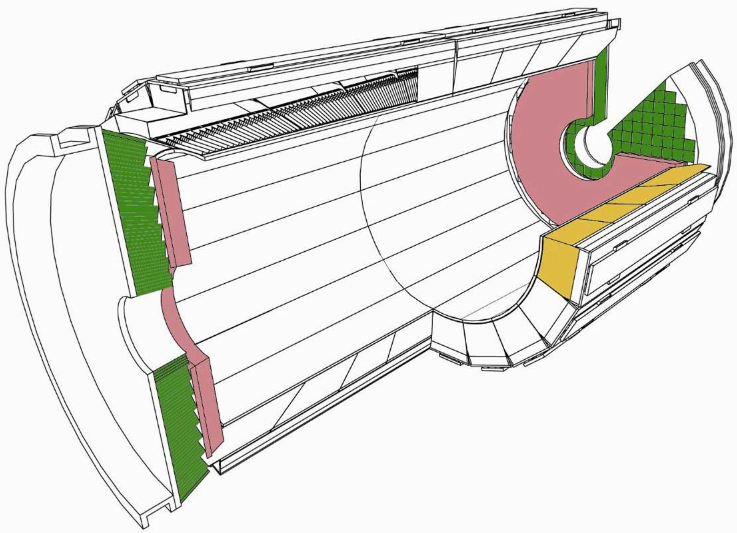
\includegraphics[width=0.8\textwidth]{figures/ecalBarrelEndcapAndPreshower.png}
	\caption{The ECAL barrel, endcap and preshower detectors.}
	\label{fig:ecalEBEEandES}
\end{figure}

%Hadrons that impinged on the HCAL showered in metal absorber layers, and in $\sim$10 ns produced scintillation 
%light in the plastic tiles.  Optical fibers transmitted the scintillation light to hybrid photodiodes, 
%which measured the scintillation light to determine the energies of incident hadrons.  The HCAL was used in 
%combination with the tracker, ECAL, and muon detectors to measure the energy of jets.  After calibrating the 
%HCAL and the other sub-detectors, the energy of jets with $\pt > 50\GeV$ and $|\eta| < 3.0$ was measured with 
%a resolution better than 15\% \cite{jetResolutionInCollisions}.

Photons and electrons that impinged on the ECAL interacted with lead-tungstate nuclei, causing a scintillation 
signal to be emitted that was detected with avalanche photodiodes in the barrel, and vacuum phototriodes in the 
endcap.  The density of PbWO$_{4}$, 5.4 $\frac{gm}{cm^{3}}$, 
was sufficiently high that the scintillation signal was usually fully contained in a 3 $\times$ 3 crystal 
grid centered on the most energetic crystal.  PbWO$_{4}$ was chosen because the scintillation signal was fast - 
more than 80\% of the scintillation light was emitted in $\sim$20 ns - as required by the high pp collision rate.  
The scintillation signal was amplified and measured by photodetectors to determine the energy of incident 
photons and electrons.  Based on real collision data, the ECAL measured the energies of electrons from $Z \rightarrow ee$ 
decays ($\Et \approx 45 \GeV$) with a resolution better than 2\% for $|\eta| < 0.8$, and between 2\% and 5\% elsewhere.  
At a slightly lower $\Et$ scale in real collision data, the ECAL measured the energies of photons from $Z \rightarrow \mu\mu\gamma$ 
decays with a resolution of 2.5\% in the barrel, and 4.7\% in the endcaps \cite{ecalPerformanceInCollisions}.

To maintain the ECAL energy resolution, the ECAL crystals were monitored and calibrated 
during data taking using several techniques.  Every 40 minutes each ECAL crystal was illuminated 
with light from blue and green lasers to monitor the crystal transparency.  Every week laser data 
was used to calculate new crystal correction factors, which corrected the changes in crystal transparency 
since the previous week.  Photons from $\eta \rightarrow \gamma\gamma$, and electrons from 
$W \rightarrow e\nu$ and $Z \rightarrow e^{+}e^{-}$ were used to validate the weekly transparency corrections.

To compliment the transparency corrections, additional corrections were applied to ECAL crystals 
to calibrate their responses based on the arrival times and energies of reconstructed particles.  Relative energy 
and relative arrival time corrections were calculated from 
the weighted average correction determined from methods described elsewhere \cite{eGammaMonitCalib2011}.  
The relative corrections normalized the responses of all crystals, in terms of energy and time, to the same value, then 
absolute energy scale corrections were applied.  The absolute energy correction for each crystal was derived using 
electrons from $Z \rightarrow e^{+}e^{-}$, and ensured the average dilepton mass measured by each crystal in 
$Z \rightarrow e^{+}e^{-}$ events was consistent with the true $Z$ boson mass.  New arrival time corrections 
were applied every month, and new energy corrections were applied once in September 2015.

During particle reconstruction energies measured by individual ECAL crystals were grouped into dynamically 
sized superclusters (SCs) with at least 9 crystals.  The SC size was allowed to vary to capture bremsstrahlung 
photons produced by electrons traversing the silicon tracker.  In the subset of SCs that were isolated 
from HCAL energy deposits, each $e^{\pm}$ was identified as a SC that geometrically matched a reconstructed track 
trajectory, and each photon was identified as a SC not matched to any track.


\section{The Hadronic Calorimeter}
\label{sec:hcalDescription}
Surrounding the ECAL was the hadronic calorimeter (HCAL), which detected charged and neutral hadrons.  The 
HCAL is a sampling calorimeter constructed with 17 layers of 3.7 mm thick scintillating plastic tiles separated by 
17 layers of metal absorber plates about 5 cm thick.  In the barrel 
region ($0 < |\eta| < 1.4$), absorber plates and scintillating tiles were organized into 2304 towers, each 
covering a 5 $\times$ 5 grid of ECAL barrel crystals.  In the endcap region ($1.3 < |\eta| < 3.0$), absorber 
plates and scintillating tiles were assembled into 2304 towers (1152 per endcap), each covering 
a 5 $\times$ 5 grid of ECAL endcap crystals.

Hadrons that impinged on the HCAL showered in metal absorber layers, and in $\sim$10 ns produced scintillation 
light in the plastic tiles.  Optical fibers transmitted the scintillation light to hybrid photodiodes, 
which measured the scintillation light to determine the energies of incident hadrons.  The HCAL was used in 
combination with the tracker, ECAL, and muon detectors to measure the energy of jets.  After calibrating the 
HCAL and the other sub-detectors, the energy of jets with $\pt > 50\GeV$ and $|\eta| < 3.0$ was measured with 
a resolution better than 15\% \cite{jetResolutionInCollisions}.

To maintain the energy resolution of the HCAL, the amount of light measured in scintillating tile towers 
was monitored and calibrated before and during 2015 collisions.  Before collisions, a radioactive source 
with known radioactivity was lowered into the HCAL, and the amount of scintillation light produced by each 
tower was used to calibrate each tower's response.  Once collisions began, a laser system 
monitored the efficiency of light transmission from the scintillator tiles to the photodetectors.  
From laser transparency data, relative calibrations were derived that normalized the response of all towers 
to the same level.  The absolute 
calibration was determined in events where a jet recoiled off a photon, or a leptonically decaying Z boson.  
There, the absolute hadronic energy 
scale was calibrated relative to the electromagnetic or muonic energy scale derived from $Z \rightarrow \ell\ell$ 
and $Z \rightarrow \mu\mu\gamma$ events.  Finally, the precision of the absolute hadronic energy scale calibration 
was improved using dijet resonances like $W/Z \rightarrow jj$.

During particle reconstruction the energy measured by each HCAL tower was treated as the basic unit of HCAL energy.  
Each reconstructed hadron contained at least one HCAL energy deposit, and potentially one or more ECAL energy 
deposits.  Charged hadrons were identified as calorimeter energies geometrically matched to reconstructed 
track trajectories, while neutral hadrons were identified as calorimeter energy deposits not matching any 
track.


\section{The Muon Detectors}
\label{sec:muonDetectorsDescription}
Interspersed among layers of the magnet iron return yoke were gas ionization chambers used to detect muons.  Muons 
that traversed the chambers ionized charge along their trajectories, and the ionized charges drifted to the 
anodes and cathodes.  The muon detectors measured the momenta, trajectories, and arrival times of muons with $0 < |\eta| < 2.4$ by 
measuring the amount of charge collected by the anodes and cathodes.  The muon detectors measured each muon's arrival 
time to identify the collision event that produced it.

The muon barrel and endcap sections, shown in Figure \ref{fig:muonBarrelAndEndcapDetectors}, used three types of 
gas ionization detectors to measure muon momenta, trajectories, and arrival times.  In the barrel region ($0 < |\eta| < 1.2$), 
drift tubes (DTs) and resistive plate chambers (RPCs) measured muon momenta, trajectories, and arrival times.  In 
the endcap region ($1.2 < |\eta| < 2.4$), RPCs and cathode strip chambers (CSCs) measured the same quantities.

\begin{figure}[ht]
	\centering
	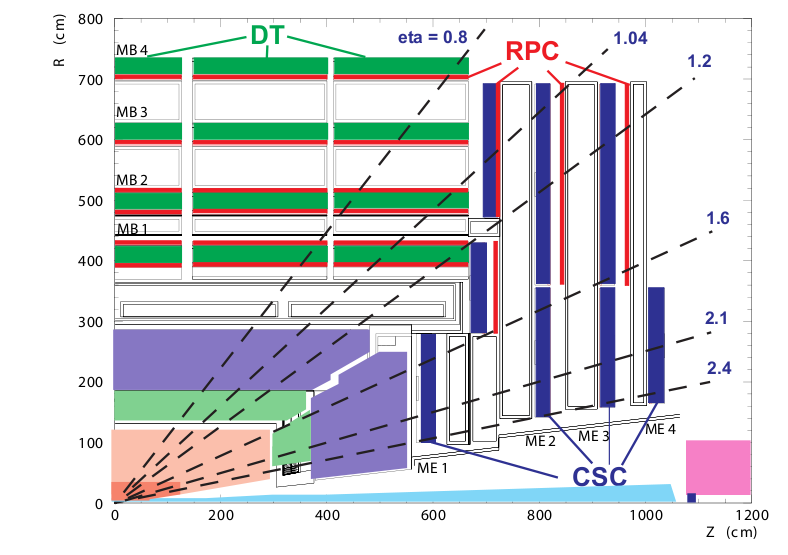
\includegraphics[width=0.8\textwidth]{figures/muonDetectorLayout.png}
	\caption{The barrel and endcap sections of the muon detectors for $\eta \geq 0.$ and one quadrant of $\phi$.  Shown 
		between the muon detectors and the interaction point are the magnet solenoid and return yoke, the HCAL, the ECAL, 
		and the silicon tracker.}
	\label{fig:muonBarrelAndEndcapDetectors}
\end{figure}

The DTs were organized into 5 wheels, each with 4 radial layers or 'stations', and 12 $\phi$ segments per 
station covering 30 degrees in $\phi$.  Each DT chamber contained several planes of drift tubes to measure 
muon trajectories in $z$, and r-$\phi$.  Using these planes, in 2015 collisions each DT station measured muon trajectories 
with a resolution better than 300$\mu$m in any direction, and measured muon arrival times with a resolution of 2 ns \cite{cmsMuonRecoRunTwo}.  

In the endcap, CSCs were installed in four disks that faced the interaction point.  
The disks were segmented into several radial layers (rings of different radii, 'stations'), as shown in Figure \ref{fig:muonBarrelAndEndcapDetectors}, 
and each station contained 18 or 36 chambers with multiple measurement planes.  The CSCs measured muon trajectories with 
resolution better than 150 $\mu$m in any direction, and measured muon arrival times with a resolution of 3.2 ns.  

In the barrel and the endcap for $|\eta| < 1.9$, the RPCs measured muon arrival times with a resolution better than 
2 ns.  RPC measurements were used by the trigger system to identify the collision event that produced each muon \cite{cmsMuonRecoRunTwo}.

The muon detectors complimented measurements made by the tracker, and improved the resolution of muon 
momentum measurements for high $\pt$ muons relative to tracker only performance.  The strength of the magnetic field 
enabled the tracker to measure muon momenta in the $\pt <$ 200 $\GeV$ phase space with 3 or more times better resolution 
than the muon detectors.  As muon $\pt$ increased above 200 $\GeV$, muon trajectories approached straight line paths, 
and the tracker momentum resolution degraded.  Using cosmic ray muons detected in 2015, the combined tracker and muon 
detector system measured the $\pt$ of barrel region muons with $200 < \pt < 400 \GeV$ with a resolution better than 
3.5\% \cite{cmsMuonRecoRunTwo}.

The muon detectors measured tracks that were used in muon reconstruction.  Muons produced outside the silicon tracker 
were identified as individual tracks in muon detectors, while muons produced within the silicon tracker were identified 
as silicon tracker tracks whose trajectories extrapolated to muon detector tracks.


\section{The Trigger System}
\label{sec:triggerDescription}
In 2015 the rate of pp collision events delivered by the LHC was several orders of magnitude greater than the 
rate that CMS could process collision event data into reconstructed particles.  The LHC collided two proton bunches 
at a rate of 40 MHz, and in nearly every collision $\gtrsim$1 $\GeV$ of energy was detected in CMS.  Due to the large cross 
section of QCD multijet processes and leptonically decaying heavy quark processes (Figure \ref{fig:smProductionXsxns}), CMS 
detected $\sim10^{6}$ collision events per second with energetic charged leptons or hadronic jets.  In 2015 
CMS was able to readout all detector information and subsequently reconstruct particles in only $\sim10^{3}$ 
collision events per second, so a two level trigger 
system selected events during collisions ('online') that were reconstructed for physics analyses and detector calibration.

\begin{figure}[h]
	\centering
	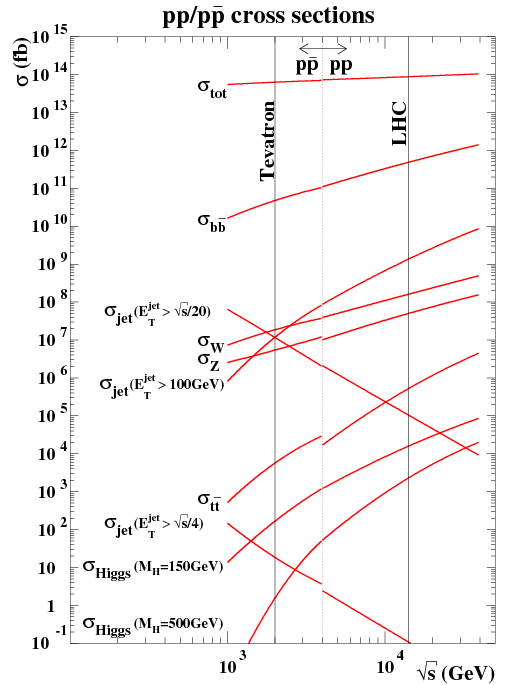
\includegraphics[width=0.6\textwidth]{figures/lhc_and_tevatron_cross_sections_2006.png}
	\caption{Production cross sections at the LHC and Tevatron as a function of center of mass energy.  Each cross section divided by $10^{5}$ yields 
	the approximate production rate in events per second in 2015 at the LHC.}
	\label{fig:smProductionXsxns}
\end{figure}

The Level-1 (L1) trigger system searched for collision events with photons, charged leptons, hadronic 
jets or neutrinos.  After every collision event, data from the ECAL, the HCAL and the muon detectors was used to build 'trigger 
primitive' objects that represented photons, muons and other particles.  In $\sim$1 $\mu$s these objects, 
distinguished by $\Et$ values and $(\eta, \phi)$ coordinates, were built and sent to the L1 logic system located 
$\sim$20 m from CMS.  Implemented in programmable hardware like Field Programmable Gate Arrays, the L1 
logic system ran $\sim$200 algorithms in less than 1 $\mu$s, and identified trigger primitive objects passing $\Et$ 
and $|\eta|$ selections.  Approximately 80000 events per second were found with at least one trigger 
primitive object passing selections, and these events were processed by the second level trigger.  

The second level, or High Level, trigger (HLT) selected events for offline reconstruction and subsequent 
use in physics analyses and detector calibration analyses.  The HLT began by transferring data from all 
sub-detectors to multi-core processors running the HLT software.  
A fast, simplified version of the full offline particle reconstruction software was run in small 
regions where L1 trigger algorithms had fired.  Then, $\sim$400 different selection algorithms, running in 
parallel, applied selections ($\Et$, $|\eta|$, etc) to locally reconstructed particles 
to identify energetic photons, charged leptons, jets, and neutrinos.  Events that passed at least one selection 
algorithm, approximately 1000 events per second, were subsequently processed by the full offline reconstruction 
software described next.

%Considering events selected by any HLT algorithm, during 2015 pp collisions the rate of data written to 
%permanent storage was $\lesssim 0.5$ gigabytes per second.

